\section{Formulation}

The \gls{good} model represents the bulk power system in physical and policy terms. The \gls{good} model contains two fundamental components:

\begin{enumerate}
	\item \textbf{Power System Graph} The power system is defined by the directed graph $G = \{R, E\}$ where $R$ is the set of regions and $E$ is the set of transmission connections between regions. Each node $r \in R$ has a set of assets $\Theta(A, r) \subseteq A$ where $A$ is the set of assets in the model. Assets are generators, stores, and loads which add or subtract energy from the system. Assets must belong to exactly one region. Balancing regions are connected to one-another via transmission edges containing transmission lines. Each edge $(i, j) \in E$ has a set of lines $\Psi(\Lambda, i, j) \subseteq \lambda$ where $\Lambda$ is the set of lines in the model.
	\item \textbf{Policy Set} Policies are contained in the set $P$ where each policy $p \in P$ applies to a set of assets $\Phi(A, p) \subseteq A$. Policies serve to favor certain classes of asset over others. Policies apply to groups of assets which may include assets which may be from multiple balancing regions. Multiple policies may apply to a single asset. Assets may belong to multiple policies.
\end{enumerate}

The physical and policy components interact to effect the optimal dispatch of grid assets and transmission lines contributing to an overall system cost. The objective of the \gls{good} model is to produce an optimal set of operational (\gls{od}) and strategic (\gls{ce}) variables such that overall cost is minimized subject to constraints. Constraints are at the asset level (maximum output, ramp rate, maximum capacity, etc.), the energy system level (energy balance, transmission limits), and the governance level (\gls{rps}). An example schematic structure is provided in Figure \ref{fig:physical_schematic}.

\begin{figure}[H]
	\centering
	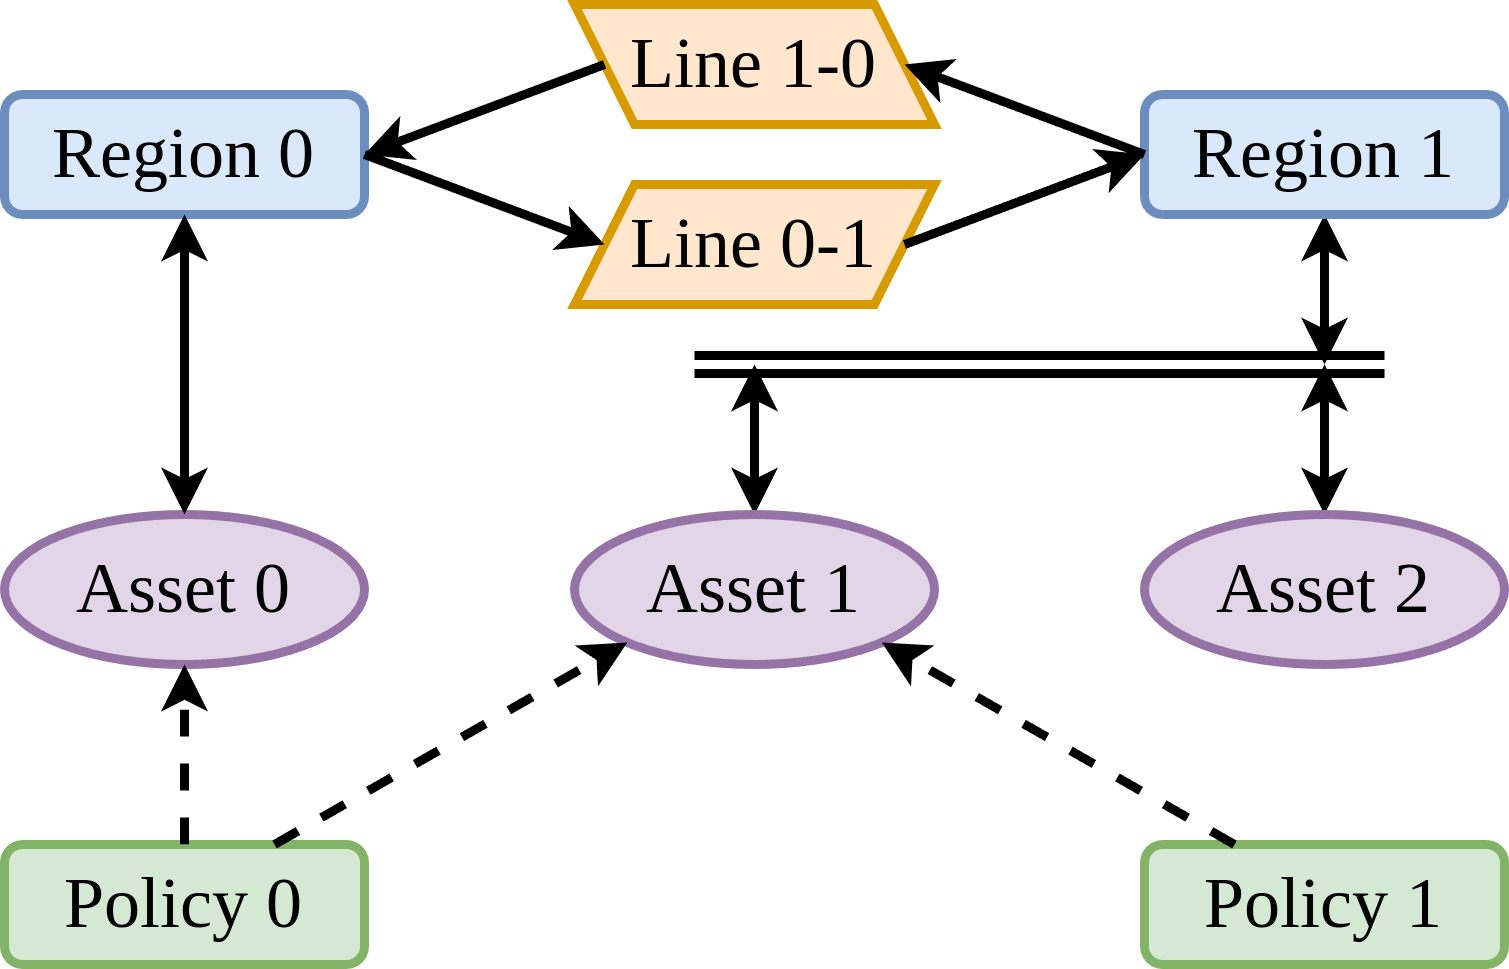
\includegraphics[width = .67\linewidth]{figs/physical_schematic.png}
	\caption{Physical schematic for an simple model. Solid arrows represent bidirectional electrical connections, double lines represent a common electrical bus, and dashed lines represent policy connections.}
	\label{fig:physical_schematic}
\end{figure}

Assets within a region are modeled as connecting with one-another and the region via a distribution system modeled as a common bus with no losses. Regions interact with one-another via directed transmission edges with losses. Policy jurisdiction do not necessarily overlap with balancing regions and, as such, policies may impact assets from multiple regions and multiple policies may impact a single asset.

\subsection{Sets}

The \gls{good} model uses the following sets:

\begin{itemize}
	\item $T$ - Time steps of the model. The steps $t \in T$ are times rather than intervals and may be unevenly spaced.
	%	\begin{itemize}
		\item $\Delta$ - Differences between time steps ($|\Delta| = |T| - 1$)
		%	\end{itemize}
	\item $U$ - Time periods in the model. Time periods $u \in U$ are sets of consecutive time steps. Time periods may overlap.
	\item $A$ - Assets such as dispatchable generators and renewables, stores, loads, and shift-able loads which add or subtract energy from the system. Each asset $a \in A$ must belong to exactly one region and may belong to zero or any number of policies.
	\begin{itemize}
		\item $A_P$ - Assets of the Producer type such as generators.
		\item $A_L$ - Assets of the Load type such as solar farms.
		\item $A_S$ - Assets of the Store type such as batteries.
	\end{itemize}
	\item $\Lambda$ - Lines which move energy from a source to a target. Lines $\lambda \in \Lambda$ belong to exactly one edge.
	\item $R$ - Balancing regions in the model. Balancing regions are the nodes of Power System graph $G$ and serve to enforce the power balance constraint considering all regional assets and inter-regional transmission. $\Omega$ and $\Delta$ are aliases for $R$ representing transmission origins and destinations respectively.
	\begin{itemize}
		\item $\Theta(A, r) \subseteq A$ Assets that belong to region $r \in R$
	\end{itemize}
	\item $E$ - Transmission edges between regions which represent the totality of transmission links between origin and destination regions. A transmission edge $(i, j)$ exists between each origin region $o \in \Omega$ and each destination region $d \in \Delta$ whether or not any lines exist along the edge. $E$ is directed $(i, j) \neq (j, i)$. Edges may contain zero or any number of lines. Edge $(o, d)$ must exist for any lines to exist between $o$ and $d$.
	\begin{itemize}
		\item $\Psi(\Lambda, i, j) \subseteq \Lambda$ - Lines that belong to edge $(i, j) \in E$
	\end{itemize}
	\item $P$ - Active policies in the model. Policies apply to specific assets which may or may not belong to the same region.
	\begin{itemize}
		\item $\Phi(A, p) \subseteq A$ Assets that belong to policy $p \in P$
	\end{itemize}
	\item $X$ - Set of time-indexed (operational) decision variables and parameters. Superscripts are used to differentiate variables in $X$ and subscripts are used to differentiate by time-step.
	\item $Y$ - Set of universal decision variables and parameters which apply at all time-steps. Superscripts are used to differentiate variables in $Y$.
	\item $Z$ - Set of investment-period-indexed (strategic) decision variables and parameters. Superscripts are used to differentiate variables in $Z$ and subscripts are used to differentiate by investment-period.
	\begin{itemize}
		\item $\hat{Z}$ - Set of initial values of variables and parameters in $Z$.
	\end{itemize}
	\item $C$ - Set of constant costs applied to variables and parameters. Superscripts correspond to variable and parameter superscripts.
	\item $H$ - Set of efficiencies applied to variables and parameters. Superscripts correspond to variable and parameter superscripts.
\end{itemize}

\subsection{Objective Function}

The goal of the optimization is to minimize the total cost of the power system considering universal, strategic, and operational costs. All costs are treated as representative present values without explicit adjustments for discounting or amortization. the user should account for these effects by setting the multipliers in $C$ accordingly.

\begin{gather}
	\min_{\overline{X}, \overline{Y}, \overline{Z}} \ \left[J_X(X) +  J_Y(Y) + J_Z(Z) \right]\label{eq:min} \\
	\begin{gathered}	
		J_X(X) = \underbrace{\sum_{t \in T}\sum_{r \in R} [c^{sr}_t x^{sr}_{t} + c^{wr}_t x^{wr}_{t}]}_{\text{Shortfall and Wastage}} + \underbrace{\sum_{t \in T}\sum_{p \in P} c^{cp} x^{cp}_t}_{\text{Compliance}} + \\\underbrace{\sum_{t \in T}\sum_{r \in R}\sum_{a \in \Theta(A, r)} \left[c^{ga}_t x^{ga}_t - c^{ea}_t x^{ea}_t \right]}_{\text{Asset Operation}} + \underbrace{\sum_{t \in T}\sum_{(i, j) \in E}\sum_{\lambda \in \Psi(\Lambda, i, j)} c^{t\lambda}_t x^{t\lambda}_t}_{\text{Line Operation}}\label{eq:jx} 
	\end{gathered}\\
	J(Y) = 0 \label{eq:jy} \\
	J_Z(Z) = \underbrace{\sum_{r \in R}\sum_{a \in \Theta(A, r)} c^{ia} z^{ia}}_{\text{Asset Initial}} + \underbrace{\sum_{(i, j) \in E}\sum_{\lambda \in \Psi(\Lambda, i, j)} c^{i\lambda} z^{i\lambda}}_{\text{Line Initial}}\label{eq:jz}
\end{gather}

The overall cost function, expressed in \eqref{eq:min}, minimizes overall costs. Operational costs, expressed in  \eqref{eq:jx}, are the sum across time-steps $T$ of the sum of regional shortfall $x^s$ and wastage $x^w$, policy compliance $x^c$, asset generation $x^{ga}$, asset expenditure $x^{ea}$ and line transmission $x^{t\lambda}$. Shortfall and wastage are optional variables which serve to penalize failure to balance energy in a region and, thus, allow for soft enforcement of the regional balancing constraint. Compliance costs serve to penalize failing to meet a policy constraint and allow for soft enforcement of the constraint. Operations for assets and lines include energy production, consumption, and transmission. Strategic costs, expressed in \eqref{eq:jz}, are the sum of asset capacity expansion $z^{ia}$ and line capacity expansion $z^{i\lambda}$. Optimization is subject to the following constraints.

\subsection{Regional Power Balance}

For each region and at each time step, the sum of power produced and consumed by assets and transmitted in and out by lines, and the values of the slack variables shortfall and wastage must equal zero. The regional power balance constraint is written as

\begin{gather}
	\underbrace{\sum_{a \in \Theta(A, r)} \left[x^{ga} + x^{ea}\right]}_{\text{Assets}} + \underbrace{\sum_{\omega \in \Omega}\sum_{\lambda \in \Psi(\Lambda, \omega, r)} \eta^{t\lambda}x^{t\lambda}}_{\text{Transmission In}} - \underbrace{\sum_{\delta \in \Delta}\sum_{\lambda \in \Psi(\Lambda, r, \delta)} x^{t\lambda}}_{\text{Transmission Out}} + \underbrace{x^{sr}_t - x^{wr}_t}_{\text{Slacks}} = 0 \quad \forall\ r \in R, \ t\in T
\end{gather}

where $\eta \in H$ are efficiencies applied to incoming transmission. Efficiencies are only applied at the receiving region. Shortfall and wastage are slack variables which do not represent physical quantities. They serve to allow for infeasible solutions to be produced. This functionality allows users the option to discover when and where infeasibility occurs for debugging purposes and to determine how much might need to be changed in order to obtain a feasible solution. Shortfall and wastage may be priced at infinity or fixed at zero to prevent infeasible solutions. Shortfall and wastage in region $r$ are constrained as

\begin{gather}
	x^{sr} \leq y^sr \\
	x^{wr} \leq y^wr
\end{gather}

where $y^{sr}$ and $y^{wr}$ are limits on allowable shortfall and wastage.


\subsection{Policies}

Operational and strategic variables may be impacted by policies. A policy may be defined in terms of operational variables (production) or strategic variables (capacity expansion). Policies may specify a ratio between a set of included assets and a set of excluded assets (proportional) or may specify a gross amount from the included set (absolute). Each policy $p \in P$ has an included set $\Phi_I(A, p) \subseteq \Phi(A, p)$ and an excluded set $\Phi_E(A, p) \subseteq \Phi(A, p)$ where $\Phi_I(A, p) \cup \Phi_E(A, p) = \Phi(A, p)$ and $\Phi_I(A, p) \cap \Phi_E(A, p) = \emptyset$. Each policy applies for a single time period $u \in U$ which consists of a set of consecutive time steps.

A policy constraint can be defined in the following ways:

\begin{description}
	\item[Proportional-Operational] \begin{equation}
		\underbrace{\sum_{t \in u}\sum_{a \in \Phi_I(A, p)} x^{ga}_t}_{\text{Included Production}} - \rho \underbrace{\sum_{t \in u}\sum_{a \in \Phi_E(A, p)} x^{ga}_t}_{\text{Excluded Production}} \geq 0
	\end{equation}
	\item[Proportional-Strategic] \begin{equation}
		\underbrace{\sum_{a \in \Phi_I(A, p)} \left[\hat{z}^{ia} + z^{ia}_u\right]}_{\text{Included Capacity}} - \rho \underbrace{\sum_{a \in \Phi_E(A, p)} \left[\hat{z}^{ia} + z^{ia}_u\right]}_{\text{Excluded Capacity}} \geq 0
	\end{equation}
	\item[Absolute-Operational] \begin{equation}
		\underbrace{\sum_{t \in u}\sum_{a \in \Phi_I(A, p)} x^{ga}_t}_{\text{Included Production}} - \gamma \geq 0
	\end{equation}
	\item[Absolute-Strategic] \begin{equation}
		\underbrace{\sum_{a \in \Phi_I(A, p)} \left[\hat{z}^{ia} + z^{ia}_u\right]}_{\text{Included Capacity}} - \gamma \geq 0
	\end{equation}
\end{description}

Existing capacities are universal parameters and members of the set $Y$. The parameters $\rho$ and $\gamma$ set the ratio or absolute value point for the policies. Typical \gls{rps} policies are Proportional-Operational with the included set composed of renewable generation assets and the excluded set composed of fossil-fuel generation assets. Less commonly found are Capacity-Absolute policies where the included set is composed of renewable generation assets. The other types are not currently found in the US.

\subsection{Components}

\subsubsection{Producers}

Producers are dispatchable assets which contribute power to the grid and receive dispatch variables at every time-step. Generator plants, river hydroelectric plants, and curtailed renewables may be modeled as producers. Producers receive a time-indexed production variable, a production cost and limit which may also be time-indexed, and a ramp-rate limit. Production is constrained as

\begin{gather}
	0 \leq x^{ga}_t \leq y^{ga}_t\quad \forall\ a \in A_P,\ t \in T \\
	-y^{ra} \left(\hat{z}^{ia} + z^{ia}\right) \leq \left(x^{ga}_t + x^{ga}_{t - 1}\right) \leq y^{ra} \left(\hat{z}^{ia} + z^{ia}\right)\quad \forall\ a \in A_P,\ t \in T \setminus \{t_0\}
\end{gather}

where $y^{ga}_t$ is the generation limit for the asset at time-step $t$ and $y^{ra}$ is the maximum allowable ramp rate. Producers receive a capacity expansion variable with an associated cost and limit. Producer capacity is constrained as

\begin{gather}
	0 \leq z^{ia} \leq y^{ia}\quad \forall\ a \in A_P
\end{gather}

where $y^{ia}$ is the limit on capacity expansion.

\subsubsection{Loads}

Loads are non-dispatchable assets which contribute power to or remove power from the grid. Solar farms, wind farms, and household load may be modeled as loads. Loads receive a capacity expansion variable with an associated cost and limit. Load capacity is constrained as

\begin{gather}
	0 \leq z^{ia} \leq y^{ia}\quad \forall\ a \in A_L
\end{gather}

where $y^{ia}$ is the limit on capacity expansion.

\subsubsection{Store}

Stores are assets which remove power from the grid, store energy, and contribute power to the grid. Batteries and pump-hydroelectric generators may be modeled as stores. Stores receive time-indexed variables production and consumption (discharging and charging) as well as limits which may be time-indexed. Stores accumulate energy and track storage level. Storage level must remain between a lower and upper bound at all ties and stores also must comply with an initial and final final value for storage level. Store operation is constrained as

\begin{gather}
	x^{\mu a}_t - x^{\mu a}_{t - 1} - x^{ga}_t\delta_{t - 1} + x^{ea}_t\delta_{t - 1} = 0\quad \forall\ a \in A_S,\ t \in T\setminus \{t_0\} \\
	0 \leq x^{\mu a}_t \leq (\hat{z}^{ia} + z^{ia}) \quad \forall\ a \in A_S,\ t \in T \\
	x^{\mu a}_0 - y^{\mu a}_0 = 0 \\
	x^{\mu a}_n - y^{\mu a}_n = 0 \\
	0 \leq x^{ga}_t \leq y^{ga}_t\quad \forall\ a \in A_S,\ t \in T \\
	0 \leq x^{ea}_t \leq y^{ea}_t\quad \forall\ a \in A_S,\ t \in T
\end{gather}

where $x^{\mu a}$ is the storage level for store $a$, $y^{\mu a}_0$ is the initial storage level,  $y^{\mu a}_n$ is the final storage level, $y^{ga}$ is the limit on production, and $y^{ea}$ is the limit on consumption.

\subsubsection{line}

Lines serve to transfer power from one balancing area (source) to a second balancing area (target). Lines receive a time-indexed transmission variable as well as a cost and limit which may also be time-indexed. Transmission is constrained as

\begin{gather}
	0 \leq x^{t\lambda}_t \leq y^{t\lambda}_t\quad \forall\ a \in A_P,\ t \in T
\end{gather}

where $y^{t\lambda}$ is the transmission limit.